Unternehmen haben strategische Ziele welche erreicht werden müssen, um Konkurrenzfähigkeit zu erhalten. Um Ziele zu erreichen werden Prozesse wie z. B. Projekte umgesetzt. Um diese zu steuern und zu kontrollieren, ist eine Form von Management notwendig, die passend zu der Unternehmensgröße und der Arbeitsweise des Unternehmens gewählt ist. Im Folgenden werden verschiedenen Anforderungen an das Management von Unternehmen dargestellt und die daraus resultierenden Methoden und Konzepte erläutert.

\subsection{Agilität}
Agilität im Kontext von Projektmanagement oder auch grundsätzlicher Unternehmensorganisation ist ein alternativer Ansatz für die Planung unternehmensinterner Prozesse, wie z. B. die Umsetzung eines Projekts und steht meist dem sogenannten traditionellen Ansatz gegenüber. Unter diesem traditionellen Ansatz wird für gewöhnlich der lineare Planungsprozess verstanden, welcher voraussetzt, dass alle Anforderungen vor der Umsetzung klar und eindeutig definiert und dokumentiert sind und somit Risiko minimiert wird. Diese Umstände sind allerdings häufig nicht gegeben, bevor ein geplanter Prozess beginnen muss, damit Konkurrenzfähigkeit für ein Unternehmen erhalten werden kann. Solche zeitkritischen Prozesse sind häufig aber maßgebend für den Erfolg eines Unternehmens, wodurch ein Bedarf für eine Methode entstand, die Anpassbarkeit an sich ändernde Anforderungen und Rahmenbedingungen während der Umsetzung eines Prozesses erlaubt \cite{agilismVsTranditionalApproaches}.

Bei traditioneller Planung erhöht sich durch sich ändernde Anforderungen das Risiko die falschen Dinge zum falschen Zeitpunkt zu tun. Agile Methodik  dagegen erlaubt es diese Prozesse so effektiv wie möglich zu managen, da die Planung nicht linear, sondern iterativ stattfindet, sodass dieses Risiko immer nur für eine Iteration in Kauf genommen werden muss. Durch regelmäßige Feedbackschleifen mit Stakeholdern bleibt der Fokus auf Werteorientierung, da sich ändernde Anforderungen regelmäßig bereits in den Planungsprozess der nächsten Iteration einbezogen werden. Somit entsteht eine Flexibilität und Anpassbarkeit, welche die Volatilität verringert. In agilen Projektteams gibt es keinen Projektmanager. Dies bedeutet aber nicht das es nicht die Aufgaben gibt, die typischerweise von einer solchen Rolle übernommen würden. Stattdessen werden Planungs- und Entscheidungsprozesse innerhalb des Teams von dem Team selbst übernommen. Dies setzt hoch qualifizierte und selbstorganisierte Teams voraus. Somit werden die Aufgaben eines traditionellen Projektmanagers in das Team übergeben und unter den Mitgliedern aufgeteilt oder von allen gemeinsam übernommen \cite{TheRoleofProjectManagerinAgileSoftwareTeams}.
Dadurch, dass Dinge erst dann entschieden werden, wenn es notwendig ist, ist allerdings der Gesamtaufwand und die -dauer nicht zu Beginn einschätzbar, sondern immer nur der Aufwand und die Dauer der aktuellen Iteration \cite{agilismVsTranditionalApproaches}.

Ziel bei der Wahl der Planungsmethode ist immer den Erfolg der Umsetzung des geplanten Prozesses zu maximieren.
Die richtige Wahl der Methode sollte zu Eingrenzung des Projektumfangs, schneller Lieferung, Qualitätssicherung, Kundenzufriedenheit und klarer Kommunikation an/zwischen Stakeholdern und somit zu Projekterfolg führen \cite{systemsApproachToPlanningSchedulingAndControlling}.
Dieser Projekterfolg kann in zwei Schlüsselfaktoren unterteilt werden: Projekteffizienz, welche die Kostenminimierung und die Erreichung von Projekt basierenden Zielen beschreibt, und Projekteffektivität, welche den Einfluss des Projekts auf die Erreichung größerer Unternehmensziele, die von Stakeholdern definiert werden, beschreibt \cite{relationshipBetweenProjectSuccessAndProjectEfficiency}.
Für Projekteffizienz, oder auch langfristiger Projekterfolg genannt, wurde bereits untersucht, inwiefern die Verwendung von agilen Methoden, den langfristigen Projekt erfolgt steigert. Dabei stellte sich heraus, dass gerade der Erfolg agiler Projektplanung von der Qualität der Teamarbeit abhängig ist.
Außerdem zeigte sich, dass in den meisten Fällen ein hybrider Ansatz sowohl dem traditionellen als auch dem strikt agilen Ansatz überlegen ist \cite{traditionalAndAgileOnProjectSuccess}.
\emph{Hat ein Projekt keinen Bedarf für agile Vorgehensweisen und wird dennoch agil durchgeführt, kann dies zu Verminderung der Projekteffizienz führen}.

\subsection{Agile Projektstruktur}
Um die Ziele eines agilen Ansatzes im Projektmanagement zu erreichen, muss die Struktur auch dem agilen Umsetzungsprozess gewachsen sein. Dazu muss das Projekt mit einem iterativen Gedanken geplant werden. Das Projekt muss also nicht nur als ein fertiges Produkt welches am Ende der vollständigen Umsetzung entstanden ist, sondern auch die Zwischenprodukte die am Ende jeder Iteration bereits entstanden sind, betrachtet werden. Das Ziel von agilem PM ist funktionierende Software und das so früh wie möglich, ohne das das vollständige Projekt umgesetzt werden muss. Hierzu verwendet man das Minimum Viable Product(MVP) und Minimum Marketable Features (MMF) \cite{agilesProjektmanagementImBerufsalltagMVPundMMF}.  Mit diesen funktionierenden und in sich geschlossenen Iterationen kann während der Umsetzung regelmäßig ein Feedbackprozess mit einem funktionierenden Produkt stattfinden. Diese Feedbackschleifen sind essenziell für die Erhaltung von Werteorientierung und Anpassbarkeit im Verlauf des Projekts \cite{}.
% Amorima, A. C., Mira da Silva, M., Pereira, R., & Colcalves, M. (2020). Using agile methodologies for adopting COBIT. https://doi.org/10.1016/j.is.2020.101496

Für MVP und MMF muss das Projekt bis zu einer bestimmten Granularität segmentiert werden. Hierzu verwendet man typischerweise sogenannte Epics und User-Stories. Epics sind in sich geschlossene Bestandteile des Produkts. Mehrere dieser Epics bilden zusammen mit ihrer vollständigen Umsetzung ein MVP oder MMF. Epics können anschließend in User-Stories aufgespalten werden, welche konkrete Funktionalitäten beschreiben. \cite{agilesProjektmanagementImBerufsalltagEpicsUndUserStories}

\vspace{20pt}
\begin{center}
    \begin{minipage}{0.8\linewidth}
        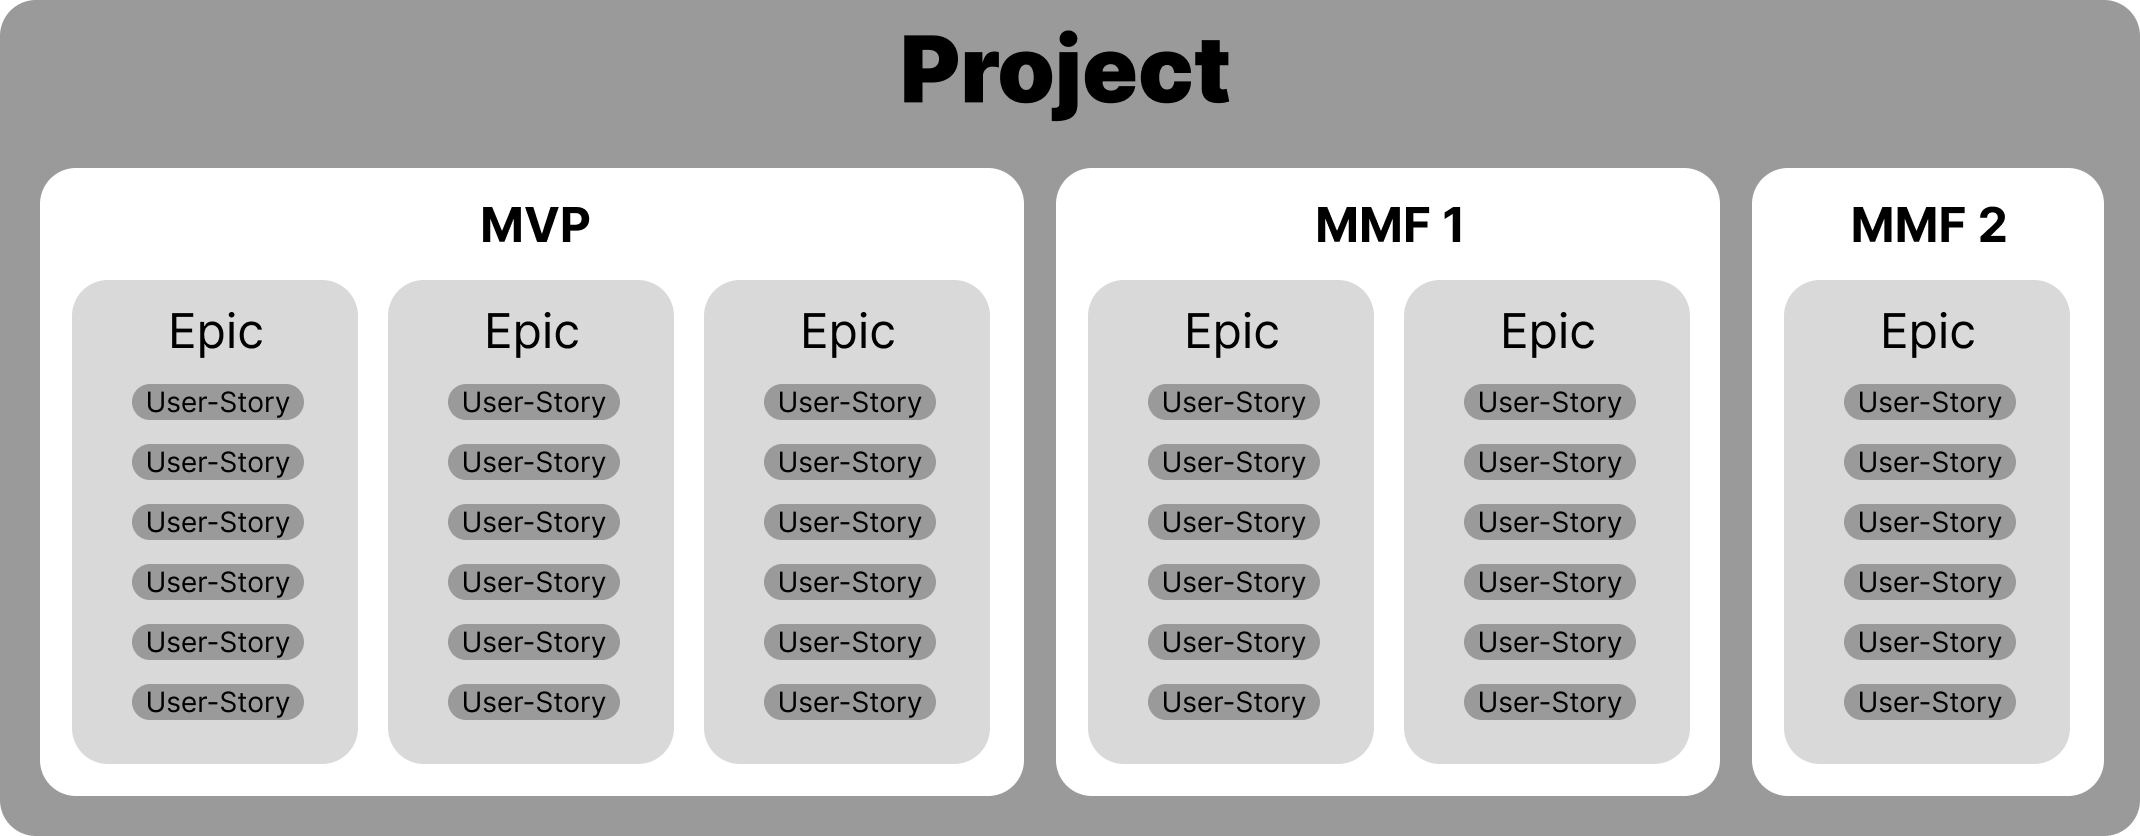
\includegraphics[width=\linewidth]{Project-Tree}
        \captionof{figure}{Agile Projektsegmentierung}
    \end{minipage}
\end{center}
\vspace{20pt}

User-Stories können zum Zeitpunkt der Umsetzung erneut in sogenannte Tasks unterteilt werden. Tasks sind Arbeitspakete die effektiv von einer einzelnen Person an einem Stück bearbeitet werden können. Diese Arbeitspakete sollten von den operativen Projektteammitgliedern definiert werden, da diese die am besten abschätzen können, wie die Beschaffenheit der Tasks sein muss, um Teamressourcen, wie Kapazität und Kompetenzen innerhalb des Teams, optimal zu nutzen. \cite{agilesProjektmanagementImBerufsalltagEpicsUndUserStories}

Für die Umsetzung gibt es verschiedene Kommunikations-Frameworks. Die beiden meist vertretenen Frameworks sind Scrum und Kanban. Beide Frameworks bieten Möglichkeiten den iterativen Umsatzprozess mit regelmäßigen Meetings, die ein konkretes Ziel verfolgen, zu strukturieren \cite{}.

\subsection{Agiles Portfoliomanagement}
Projekt Portfoliomanagement(PPM) wird traditionell dazu verwendet eine Portfolio bestehend aus Projekten innerhalb eines Unternehmens zu verwalten. Die Projekte eines Portfolios teilen sich Ressourcen und müssen koordiniert, sowie priorisiert werden \cite{NGUYEN20181054}.
% Nguyen, N. M., Killen, C. P., Kock, A., & Gemunden, H. G. (2018). The use of effectuation in projects: The influence of business case control, portfolio monitoring intensity and project innovativeness. International Journal of Project Management, 36(8), 1054–1067. Available at: https://doi.org/10.1016/j.ijproman.2018.08.005
Das Ziel dabei ist immer den finanziellen Wert über die Projekte eines oder sogar mehrerer Portfolios hinweg zu maximieren und sie dabei mit Unternehmenszielen zu verknüpfen, um die Strategie des Unternehmens in Hinsicht auf die innerhalb des Unternehmens verfügbaren Ressourcen zu verfolgen \cite{MARTINSUO200756}.
% Martinsuo, M. and Lehtonen, P. (2007). Role of single-project management in achieving portfolio management efficiency. International Journal of Project Management, 25(1), pp.56–65. Available at: https://doi.org/10.1016/j.ijproman.2006.04.002

\emph{multi agile project product and stuff}
Die Verwaltung von agilen Projekten führte dazu, dass Agilität bis auf das PPM skaliert werden kann, um Entscheidungen auf Portfolioebene ebenfalls Wertegetrieben, statt ausschließlich Ressourcen- und damit Kosten-basiert, treffen zu können. Um dies zu erreichen, gibt es ebenfalls verschiedene Frameworks, die in den folgenden Abschnitten genauer beschrieben werden \cite{SUAREZ2022-1}.
% Scalable agile Frameworks on Large Enterprise Portfolios Page 14

Vorteile der Implementierung von agilen Framework für PPM stellt bei Portfolios mit variablen und innovativen Projekten eine Möglichkeit dar, Time-to-Market, Team-Produktivität und Kommunikation zu steigern \cite{SUAREZ2022-2}.
% Scalable agile Frameworks on Large Enterprise Portfolios Page 31

Eine Studie zeigte ebenfalls, dass sich durch diese Implementierung (1) Transparenz über Ressourcen und Aufgaben erhöht und damit Vertrauen, Entscheidungsfindung und Ressourcenzuweisung verbessert wird, (2) bessere Zusammenarbeit und routinierte Interaktion zu Artefakten für die Ermöglichung regelmäßiger Feedbackschleifen führt, (3) Commitment für die Strategie des Portfolios gesteigert wird und (4) die Orientierung des Teams fokussiert wird, indem Unruhen in der Ressourcenzuweisung reduziert und potenzial der Teams erhöht \cite{anEmpiricalPerspectiveOnThePractiveInUse}.

\subsection{Agile Unternehmensstrukturierung}
Für die Skalierung von Agilität auf die gesamte Unternehmensstruktur, gibt es, wie bereits erwähnt, verschiedene Frameworks. Diese werden im folgenden Abschnitt genauer beschrieben.

\subsubsection{SAFe}
Es wurde von Dean Leffingwell entwickelt und ist eine der meistverbreiteten Methoden für agile Unternehmensstrukturierung.
SAFe unterteilt ein Unternehmen in drei bis 4 Ebenen. Diese Ebenen sind:

\begin{itemize}
    \item Team Level
    \item Program Level
    \item Value Stream Level (optional)
    \item Portfolio-Level
\end{itemize}

Das Team-Level bildet die operative Ebene in der agile Teams agieren. Diese Teams können SCRUM oder Kanban verwenden, besonders wert wird aber darauf gelegt, dass alle Teams in einem einheitlichen Iterationsintervall arbeiten.

Das Program Level fasst 5 bis 12 agile Teams aus dem Team-Level in ein virtuelles Programm zusammen, welches als Agile Release Train (ART) bezeichnet wird. Diese ARTs sind langlebige, selbstorganisierte Teams, welche gemeinsam für den Erfolg des ARTs verantwortlich sind.

Das optionale Value Stream Level ist eine Ebene, die verwendet werden kann, wenn es mehrere ARTs gibt, welche einen gemeinsamen Wertestrom ergeben und deshalb zusätzliche Koordination benötigen.

Das Portfolio-Level ist die Ebene, in der die Werteströme entweder aus dem Value Stream Level oder dem Program Level organisiert und finanziert werden. Dort finden Praktiken wie Lean-Agile Budgeting ihre Anwendung für die notwendige Kontrolle über die verschiedenen Werteströme.

Zuletzt gibt es noch die sog. Foundation Layer, welche verschiedene Richtlinien definiert, welche als Grundlage der Prinzipien hinter SAFe dienen. Dazu gehören die 9 Lean-Agile Principles, Leitlinien für agile Führungsrollen, etc. \cite{leffingwell20safe}

\subsubsection{Flight-Level}
Flight-Level ist eine weitere Methode, welche eine mögliche Form von agiler Unternehmensstrukturierung bietet und wurde von Klaus Leopold entwickelt. Die Methode Flight-Level wird hierbei von Leopold \cite{agilitaetNeuDenken} als Kommunikations-Framework bezeichnet und unterteilt ein Unternehmen in 3 Ebenen oder auch Flight-Level, also Flughöhen bezeichnet:
\begin{longtable}{p{3cm}p{10cm}}
    Flight-Level 1: & Operative Ebene mit einem Projekt oder Team \cr
    Flight-Level 2: & Koordinierung der Zusammenarbeit mehrerer Teams\cr
    Flight-Level 3: & Strategisches Portfoliomanagement.
\end{longtable}

Die verschiedenen Flight-Level sollen einen Blick in unterschiedlichen Detailgraden auf das Unternehmen ermöglichen, ähnlich wie bei einem Blick aus einem Flugzeug in verschiedenen Flughöhen. Kommunikation zwischen den Ebenen wird als kritischer Faktor dargestellt, welcher die Wertschöpfung steigern, da sich das Unternehmen besser und schneller an die Veränderungen des Marktes anpassen können soll und somit die Konkurrenzfähigkeit bewahren kann. Ähnlich wie bei agilen Projektmanagement-Frameworks, gibt diese Methode eine klare Struktur in der Kommunikation vor.